%Version 3 October 2023
% See section 11 of the User Manual for version history
%
%%%%%%%%%%%%%%%%%%%%%%%%%%%%%%%%%%%%%%%%%%%%%%%%%%%%%%%%%%%%%%%%%%%%%%
%%                                                                 %%
%% Please do not use \input{...} to include other tex files.       %%
%% Submit your LaTeX manuscript as one .tex document.              %%
%%                                                                 %%
%% All additional figures and files should be attached             %%
%% separately and not embedded in the \TeX\ document itself.       %%
%%                                                                 %%
%%%%%%%%%%%%%%%%%%%%%%%%%%%%%%%%%%%%%%%%%%%%%%%%%%%%%%%%%%%%%%%%%%%%%

%%\documentclass[referee,sn-basic]{sn-jnl}% referee option is meant for double line spacing

%%=======================================================%%
%% to print line numbers in the margin use lineno option %%
%%=======================================================%%

% \documentclass[lineno,sn-basic]{sn-jnl}% Basic Springer Nature Reference Style/Chemistry Reference Style

%%======================================================%%
%% to compile with pdflatex/xelatex use pdflatex option %%
%%======================================================%%

\documentclass[pdflatex,sn-basic, Numbered]{sn-jnl}

%%%% Standard Packages
%%<additional latex packages if required can be included here>

\usepackage{graphicx}%
\usepackage{multirow}%
\usepackage{amsmath,amssymb,amsfonts}%
\usepackage{amsthm}%
\usepackage{mathrsfs}%
\usepackage[title]{appendix}%
\usepackage{xcolor}%
\usepackage{textcomp}%
\usepackage{manyfoot}%
\usepackage{booktabs}%
\usepackage{algorithm}%
\usepackage{algorithmicx}%
\usepackage{algpseudocode}%
\usepackage{listings}%
\usepackage{multicol}

% additional packages
\usepackage{caption}
\usepackage{placeins}
\usepackage{lipsum}
\usepackage{float}
\usepackage{csquotes}
\usepackage{sidecap}
\usepackage{url}                     % fix URL wrap
\usepackage{booktabs}                % Improves the quality of tables in LaTeX
\usepackage{tabularx}                % Enhances the standard LaTeX tables
\usepackage{subcaption}              % Provides support for subfigures and subtables
\usepackage{longtable}               % Allows the creation of multi-page tables
\usepackage{multirow}                % Enables cells spanning multiple rows in tables
\usepackage{threeparttable}          % Provides additional functionality for tables
\usepackage{array}
\usepackage{eurosym}

\def\UrlBreaks{\do\/\do-}
\renewcommand{\floatpagefraction}{0.5}
\renewcommand{\textfraction}{0.1}

%% as per the requirement new theorem styles can be included as shown below
\theoremstyle{thmstyleone}%
\newtheorem{theorem}{Theorem}%  meant for continuous numbers
%%\newtheorem{theorem}{Theorem}[section]% meant for sectionwise numbers
%% optional argument [theorem] produces theorem numbering sequence instead of independent numbers for Proposition
\newtheorem{proposition}[theorem]{Proposition}%
%%\newtheorem{proposition}{Proposition}% to get separate numbers for theorem and proposition etc.

\theoremstyle{thmstyletwo}%
\newtheorem{example}{Example}%
\newtheorem{remark}{Remark}%
\theoremstyle{thmstylethree}%
\newtheorem{definition}{Definition}%

\raggedbottom
%%\unnumbered% uncomment this for unnumbered level heads

\newcommand{\comment}[1]{\textcolor{purple}{#1}}

%%=============================================================%%
%%=============================================================%%
\begin{document}

\title[Article Title]{24/7 carbon-free electricity matching accelerates adoption of advanced clean energy technologies}

%%=============================================================%%
%% GivenName	-> \fnm{Joergen W.}
%% Particle	-> \spfx{van der} -> surname prefix
%% FamilyName	-> \sur{Ploeg}
%% Suffix	-> \sfx{IV}
%% \author*[1,2]{\fnm{Joergen W.} \spfx{van der} \sur{Ploeg}
%%  \sfx{IV}}\email{iauthor@gmail.com}
%%=============================================================%%

\author*[1]{\fnm{Iegor} \sur{Riepin}}\email{iegor.riepin@tu-berlin.de}
\author[2]{\fnm{Jesse} \spfx{D.}  \sur{Jenkins}}\email{jessejenkins@princeton.edu}
\author[3]{\fnm{Devon} \sur{Swezey}}\email{dswezey@google.com}
\author[1]{\fnm{Tom} \sur{Brown}}\email{t.brown@tu-berlin.de}
\affil[1]{\orgdiv{Department of Digital Transformation in Energy Systems}, \orgname{TU Berlin}, \orgaddress{Germany}}
\affil[2]{\orgdiv{Mechanical \& Aerospace Engineering and Andlinger Center for Energy}, \orgname{Princeton University}, \orgaddress{USA}}
\affil[3]{\orgdiv{Global Energy and Climate}, \orgname{Google LLC}}

%%==================================%%
%% abstract %%
%%==================================%%

\abstract{

Commitments to 24/7 carbon-free energy matching by companies and governments create an early market for technologies that can bridge the gaps between wind and solar generation.
We argue that the commitment by a small number of companies to round-the-clock matching can spur substantial learning in these advanced technologies.
We demonstrate these benefits for two technologies: long-duration energy storage and clean firm generation.
The reduced costs from learning make 24/7 matching more attractive for other actors, leading to a virtuous circle that accelerates the time when the technologies become cost-competitive in the rest of the electricity market.
These indirect effects unlock greenhouse gas savings far beyond the direct emission reductions from initial investments, illustrating how proactive contributions from the private sector can complement governmental support for advanced energy technologies, reduce pressure on tight fiscal budgets, and accelerate decarbonization of electricity systems.
}

%########################################################################
%########################################################################

\subsection*{Highlights}

\begin{itemize}
\item 24/7 CFE matching creates an early market for advanced energy technologies
\item Early deployment of advanced technologies spurs substantial learning effects
\item Self-reinforcing system dynamics accelerate widespread adoption of advanced technologies
\item These indirect effects yield greenhouse gas savings far beyond the impact of initial investments
\item Corporate deployment via 24/7 is a viable channel for new technologies if government budgets are constrained
\end{itemize}

\subsection*{Graphical abstract}

\begin{center}
    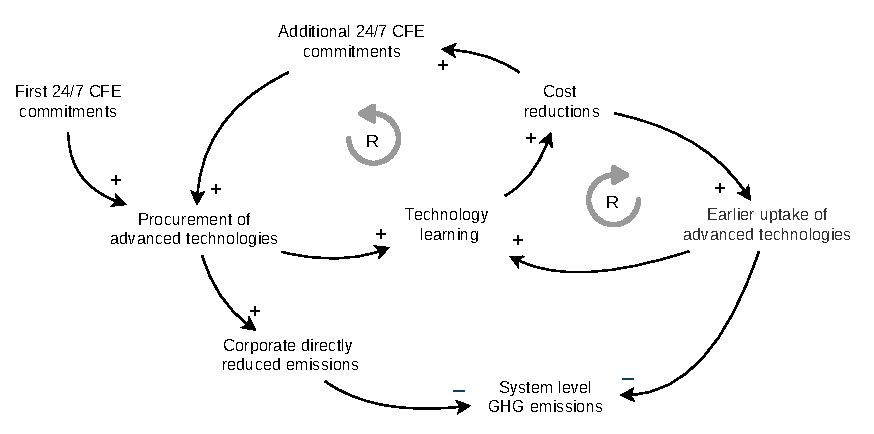
\includegraphics[width=0.85\textwidth]{images/virtuous_dynamics.pdf}
\end{center}

\subsection*{Metadata (original submission)}
\begin{itemize}
    \item Words in text: 2706
    \item Words outside text (captions): 358
    \item Number of figures: 4
    \item Number of headers: 6
    \item Number of references: 20
    \item Supplementary information: Document S1. Table S1 (Technology assumptions) Supplementary references.
\end{itemize}

\subsection*{Metadata (revision)}
\begin{itemize}
    \item Words in text: 3182
    \item Words outside text (captions): 403
    \item Number of figures: 4
    \item Number of headers: 6
    \item Number of references: 27
    \item Supplementary information: Document S1. Table S1 (Technology assumptions) Supplementary references.
\end{itemize}

\subsection*{Metadata (final version)}
\begin{itemize}
    \item Words in text: 3157
    \item Words outside text (captions): 395
    \item Number of figures: 3
    \item Number of headers: 6
    \item Number of references: 18
    \item Supplementary information: Document S1. Table S1 (Technology assumptions) Supplementary references.
\end{itemize}


%########################################################################
%########################################################################

\maketitle

\subsection*{Big challenges ahead}\label{sec1}

Tackling climate change requires not only a massive scale-up of available energy technologies like wind, solar and batteries, but also an accelerated research, development, demonstration and widespread deployment of advanced technologies that are not yet commercialised at scale \cite{sepulvedaRoleFirmLowCarbon2018, brownUltralongdurationEnergyStorage2023}.
Among them are clean firm generation technologies, such as next-generation geothermal power, advanced nuclear generators, Allam-cycle gas generators with carbon capture and storage (CCS), as well as long-duration energy storage (LDES) technologies, which can bridge multi-day gaps in clean power supply that cannot be filled by wind, solar photovoltaics (PV), or batteries.

\textbf{Barriers to commercialization---} Bringing new technologies to market on a large scale and in time, however, is fraught with challenges.
New technologies often face a \enquote{valley of death} on the path to successful commercial deployment.
Early-stage investments typically comprise governmental R\&D grants and venture capital, insufficient in both magnitude and duration to support new energy technologies \cite{khatcherianBarriersTimelyDeployment2022}. On the other hand, mature technologies such as wind and solar attract steady, de-risked capital from institutional investors.
Achieving commercial viability requires companies to construct larger plants at scale and reduce manufacturing costs, which involves overcoming financial, engineering, and supply chain issues unique to first-of-a-kind (FOAK) projects. Technology innovators often lack the resources to scale from demonstration plants to commercial-scale projects, frequently requiring a consortium of stakeholders that adds complexity and risk, complicating financing \cite{khatcherianBarriersTimelyDeployment2022}.
Even after FOAK projects succeed, scaling further remains challenging, as repeated deployments are essential for achieving economies of scale. However, investors often hesitate until proven success is seen across multiple projects. Government support can be critical here, though it can also be temporary and even unpredictable, as when Germany ended subsidies for electric cars abruptly in 2023; or in Spain, where the withdrawal of renewable energy support led numerous investors to initiate successful international arbitration proceedings against the state \cite{gurtlerDismantlingRenewableEnergy2019}. Tight public budgets can also be a limiting factor. For example, in the EU, new fiscal rules may limit member states' capacity to invest in green technologies \cite{darvasImplicationsEuropeanUnions2024}.

Overall, the road from the first demonstration plant to commercial uptake can be complicated, risky, and expensive---and it is challenging to secure the capital to fund it.

\textbf{Bridging the valley of death---} Consider how solar became a global industry and a truly disruptive technology. Bell Labs developed the first silicon photovoltaic cell in 1954, which made modern solar power possible. After more than 20 years of further development, in 1975, the Levelised Cost of Electricity (LCOE) for solar PV was above \$10,000/MWh in today's money. A historical trajectory for solar development involved Japan's niche markets for consumer electronics in the 1980s, and Germany's feed-in tariff in 2004, which created a \enquote{demand pull} leading to massive industrialization of solar PV manufacturing in China and rapid cost reduction through technological learning \cite{nemetHowSolarEnergy2019}. If we fast-forward to the 2020s, for projects with low-cost financing that tap high-quality resources, solar PV has now the cheapest levelised cost of electricity in history, with new utility-scale solar projects costing \$30-55/MWh in Europe, the US, and China \cite{ieaWorldEnergyOutlook2024}.

However, it took six decades for solar to become economically viable. The urgency of climate change mitigation demands that we accelerate this process for advanced clean energy technologies. A crucial question here: Who will invest in these technologies when they are expensive at the beginning? These investments can bring wider social benefits. New technologies, such as Allam cycle generators and iron-air battery storage, are also likely to experience cost reductions through evolving R\&D processes, learning by doing, and iterative upscaling. In this way, even though initial investments come with a price premium and certain risks, they can result in cost reductions and an earlier rollout of advanced clean energy technologies. This produces indirect effects that result in greenhouse gas savings beyond the direct reductions associated with initial investments. The key is initial investments to start this process.

In this perspective, we illustrate in the following sections how initial commitments to 24/7 Carbon-Free Energy (CFE) matching can unlock these effects.

\subsection*{The significance of 24/7 CFE matching}\label{sec2}

Many public and private energy buyers support the global effort to decarbonise electricity systems by purchasing clean energy.
Traditionally this support has consisted of buying certificates or signing power purchase agreements for renewable energy that is matched to consumption on an annual basis. 24/7 CFE is a new approach that aims to eliminate all carbon emissions by aligning electricity demand with carbon-free energy supply on \textit{an hourly basis} and on the same local grid where demand occurs.
24/7~CFE commitments were announced by large technology companies such as Google, Microsoft and Iron Mountain, as well as by utilities, and the US federal government \cite{gocarbonfree247}. The Climate Group has recently launched the 24/7 Carbon-free Coalition to encourage companies to move toward 24/7 CFE, initially comprising six companies from diverse industries---including information technology, pharmaceuticals, telecommunications, and cement---and spanning multiple geographic regions \cite{climategroup247CarbonFree2024}.

Motivated by these commitments, several quantitative studies have been conducted on the means, costs, and system-level impacts of hourly CFE matching \cite{xu-247CFE-report, riepinMeansCostsSystemlevel2024}. There are three key findings that emerge from these studies:
\begin{enumerate}
    \item 24/7 CFE commitments reduce participating buyers' emissions as well as emissions from the electricity grids where they operate.
    \item 24/7 CFE comes at a cost premium for participating consumers if only mature technologies, such as solar PV, wind, and battery storage, are used for CFE sourcing.
    \item The cost premium can be substantially reduced if participating buyers incorporate a broad range of advanced energy technologies into their procurement strategies, such as long-duration energy storage and clean firm generators.
\end{enumerate}


\begin{figure}[htbp]
    \centering
    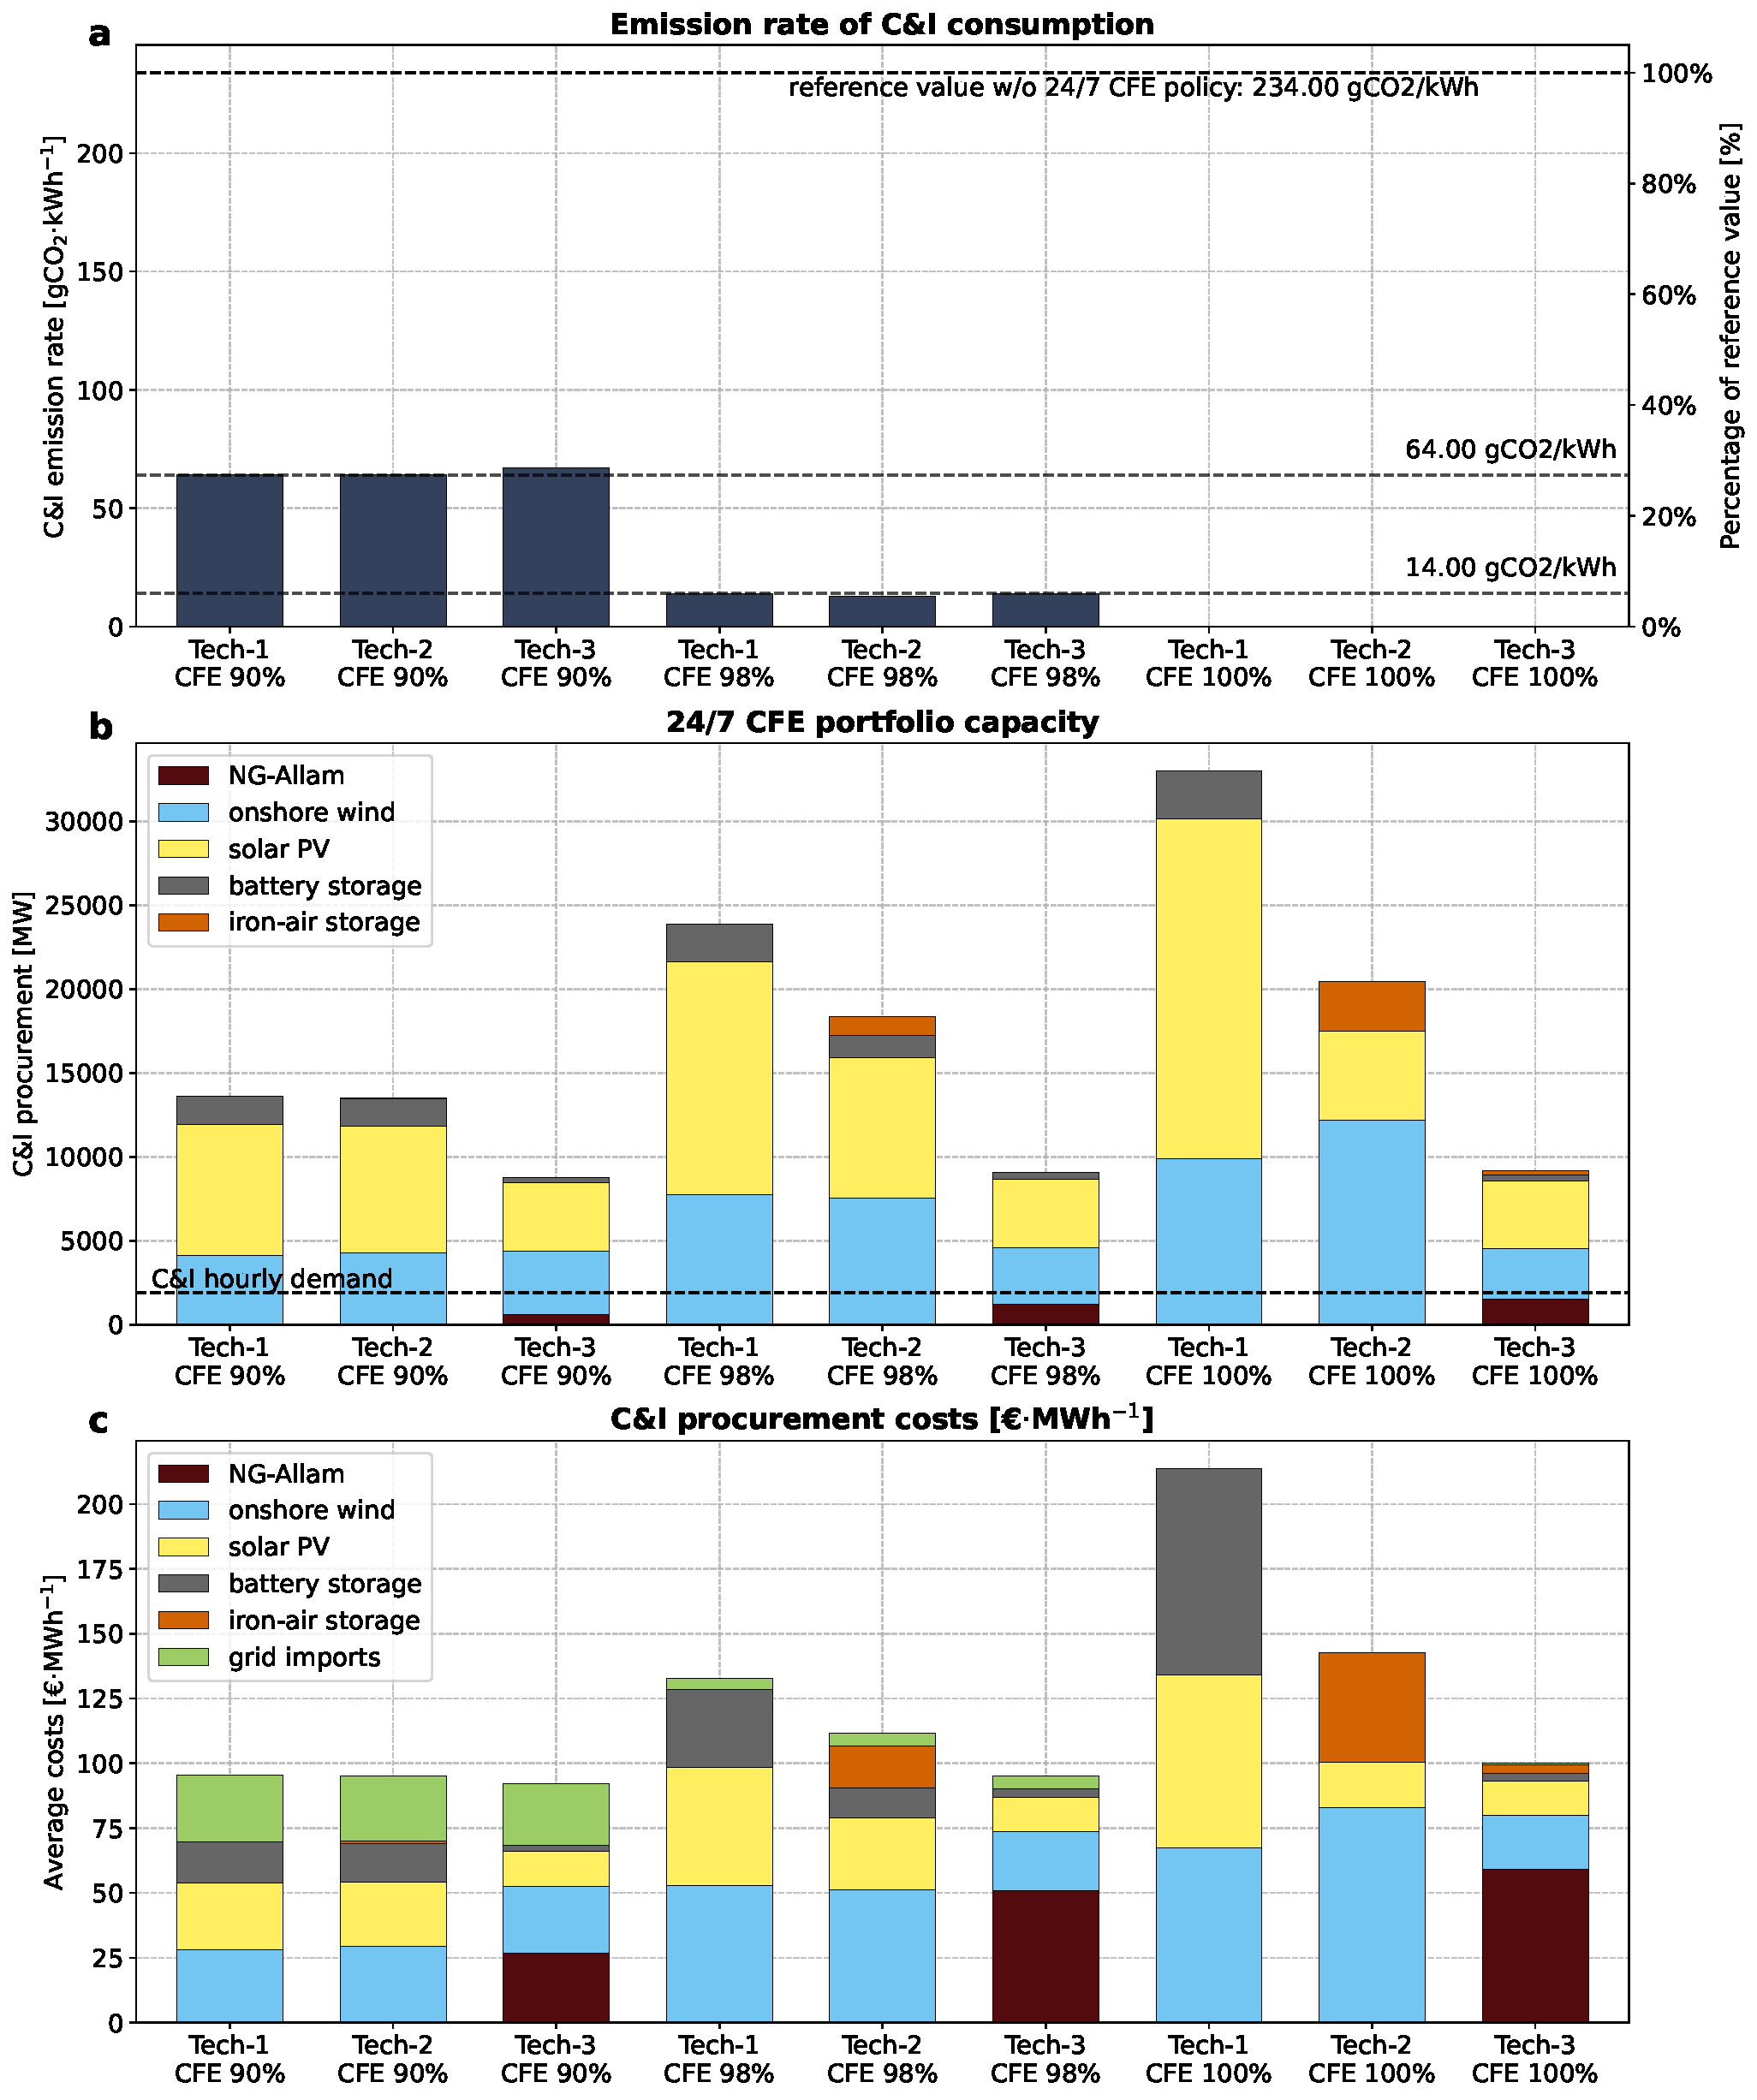
\includegraphics[width=\textwidth]{images/dashboard_247CFE.pdf}
    \captionsetup{width=\textwidth}
    \caption{Illustrative modelling of 24/7 CFE matching.
    \textbf{Panel a}: Average emissions rate of participating consumers,
    \textbf{panel b}: portfolio capacity procured by participating consumers,
    \textbf{panel c}: procurement cost by scenario.
    Here we assume Germany in 2025 as an example location and a participation rate of C\&I consumers in 24/7 CFE matching strategy at 5\% (ca. 1900~MW load).
    CFE scores of 90\%, 98\% and 100\% correspond to the share of time when the electricity consumed by the participating consumers is carbon-free.
    Technology palette 1 (\enquote{Tech-1}) comprises technologies commercially available today: onshore wind, utility scale solar PV, and battery storage; \enquote{Tech-2} includes all above plus long-duration energy storage (here: the iron-air battery as a stand-in technology); \enquote{Tech-3} includes all above plus a clean firm generator (here: the Allam cycle generator with CCS as a stand-in technology). The 24/7 CFE procurement framework is based on a methodologies paper by \citet{google-methodologies}. Simulations were carried out using the 24/7 CFE model by \citet{riepinMeansCostsSystemlevel2024}. Technology assumptions are provided in the Supplementary Information.\\
    }\label{fig:dashboard}
\end{figure}

\textbf{An illustrative example---} We demonstrate the three findings above in an example depicted in Fig. \ref{fig:dashboard}.
Here we display a situation in which a fraction of electricity demand in Germany voluntarily commits to matching their electricity demand with carbon-free electricity round-the-clock.
\textbf{Panel a} illustrates how, as the CFE target is tightened, participating consumers reduce the emission rate (gCO$_2$/kWh$^{-1}$) attributed to their electricity consumption. Once demand and supply are perfectly aligned on an hourly basis, i.e. 100\% 24/7 CFE matching is achieved, participating consumers reach emission rate of zero. This goal requires a large portfolio of wind, solar PV, and batteries, as shown in \textbf{panel b}. It is indeed difficult to match every kWh of electricity consumption with renewable electricity during times of dark wind lulls. As a result, achieving 24/7 CFE matching, including the most difficult 2\% of times, adds a high cost premium for consumers in part due to the need to build large capacities relative to the demand of participating buyers (\enquote{Tech-1, CFE 100\%}). Finding \#3 above is also clearly visible in \textbf{panel c}: the power capacity required for 24/7 CFE matching and associated costs are substantially reduced when LDES technology or clean firm generation technologies are added.

The main takeaway from this illustrative example is that 24/7 CFE matching creates an economic incentive to incorporate advanced energy technologies into procurement strategies and reduce the cost premium associated with 24/7 CFE matching. This, in turn, creates an early market for new technologies. For example, if 5\% of commercial and industrial (C\&I) consumers in Germany---representing approximately 1900~MW of load---adopt 24/7 CFE matching strategy, this would create a market for approximately 1500~MW of advanced clean firm generators and about 23~GWh of LDES (assuming all technology options are deployed, \enquote{Tech-3, CFE 100\%}).
In a similar vein to how feed-in tariffs and renewable portfolio standards created a \enquote{demand pull} for wind and solar technologies in the past, 24/7 CFE commitments can drive the deployment and accelerate innovation of advanced clean energy technologies.

\subsection*{Technology learning}\label{sec3}

The early deployment of advanced energy technologies can help them drive down along the \enquote{experience curve} -- a concept encapsulating a set of mechanisms by which technology costs decline as cumulative capacity is deployed: evolving R\&D process, learning-by-doing, incremental upscaling, economies of scale, financial innovation and experience, for example.

In this section, we analyse the expected technological learning for the two energy technologies selected as stand-ins for advanced clean firm generators and LDES: the Allam cycle generator with CCS and iron-air battery storage, respectively. The Allam cycle generator is a novel Allam-Fetvedt Cycle that uses the oxy-combustion of carbonaceous fuels and a high-pressure supercritical CO$_2$ working fluid in a recuperated cycle that by design captures nearly all emissions. The iron-air battery is a multi-day energy storage technology that uses a principle of reversible rusting to store and release energy. In practice, a wider range of long-duration storage and clean firm generation are being commercialized and are candidates for procurement under 24/7 CFE matching, including advanced nuclear fission, enhanced and closed loop geothermal energy, bioenergy with CCS, and combustion of carbon-free fuels like hydrogen, and a range of potentially low-cost electrochemical, chemical, thermal, and mechanical storage technologies.

The mathematical model of learning is based on empirical evidence in which the specific investment costs $C$ of a technology decrease by a constant factor with each doubling of experience $E$. The functional dependency is given by:

\begin{equation}
  \begin{aligned}
    \color{violet}C(E)\color{black} &= \color{blue}\overline{C_0}\color{black}  \cdot \left( \frac{\color{red}E}{\color{blue}\overline{E_0}\color{black}} \right)^{-\color{black}\alpha} \text{ where } \color{black}\alpha = \color{black}\log_2 \left( \frac{1}{1 - \color{blue}LR\color{black}} \right)
    \label{eq:learning_curve}
  \end{aligned}
\end{equation}

\noindent where the constants $\color{blue}\overline{C_0}$ [\officialeuro/kW] and $\color{blue}\overline{E_0}$ [MW] are fixed starting points representing the initial costs and experience levels, respectively. The learning rate $\color{blue}LR$ [\%] is a parameter that determines the rate at which costs decrease with experience.
If $\color{blue}LR=20\%$, the costs are reduced by 20\% for each doubling of cumulative experience.
The observed learning rates for energy technologies range from near zero (nuclear, hydropower) to 21\% (lithium-ion batteries) \cite{waySuppplementaryMaterialsEmpirically2022}; it has been shown that small, modular energy technologies have higher learning rates \cite{wilsonGranularTechnologiesAccelerate2020}.
Here we use cumulative capacity $\color{red}E$ [MW] of a technology as a proxy for experience, which is calculated as the sum of the installed capacities of all projects that have been completed by a certain point in time.
We collect information on existing and planned projects for each technology, and use this as a starting point for the experience of the technology. 24/7 CFE matching contributes to the technology's experience the additional capacity procured by participating consumers, which is proportional to the participation rate (i.e., the share of C\&I electricity demand that is matched with carbon-free electricity on an hourly basis).

The resulting investment costs $\color{violet}C(E)\color{black}$ [\officialeuro/kW] are shown in Fig. \ref{fig:panels} for Allam cycle technology (top panel) and iron-air battery storage (bottom panel).
The first 1\% of participation (around 380~MW load in the German market) reduces costs for Allam cycle generators by 12\% and iron-air storage by 16\%. The technology learning scales significantly from there: at 10\% participation, Allam cycle generators and iron-air storage costs are reduced by 38\% and 44\%, respectively. The learning effect has a diminishing return, due to the logarithmic term $\color{black}\alpha$ in Eq. \ref{eq:learning_curve}. In other words, the first projects have the most significant impact on technology learning, and the effect diminishes as technology experience grows.

The learning model is subject to uncertainty in the initial costs and experience levels, as well as the learning rate. Our Monte Carlo simulation captures this uncertainty by sampling the initial costs and experience levels based on probability distributions derived from public information about planned projects. Fig. \ref{fig:panels} displays the Monte Carlo simulation results as violin plots. Even though both technologies have a wide range of cost outcomes, the main observation is robust to uncertainty: the early deployment of advanced clean energy technologies due to 24/7 CFE commitments substantially reduces technology costs, making them more attractive for other actors and accelerating the point where the technologies become cost-competitive in the rest of the electricity system.

\begin{figure}[htbp]
    \centering
    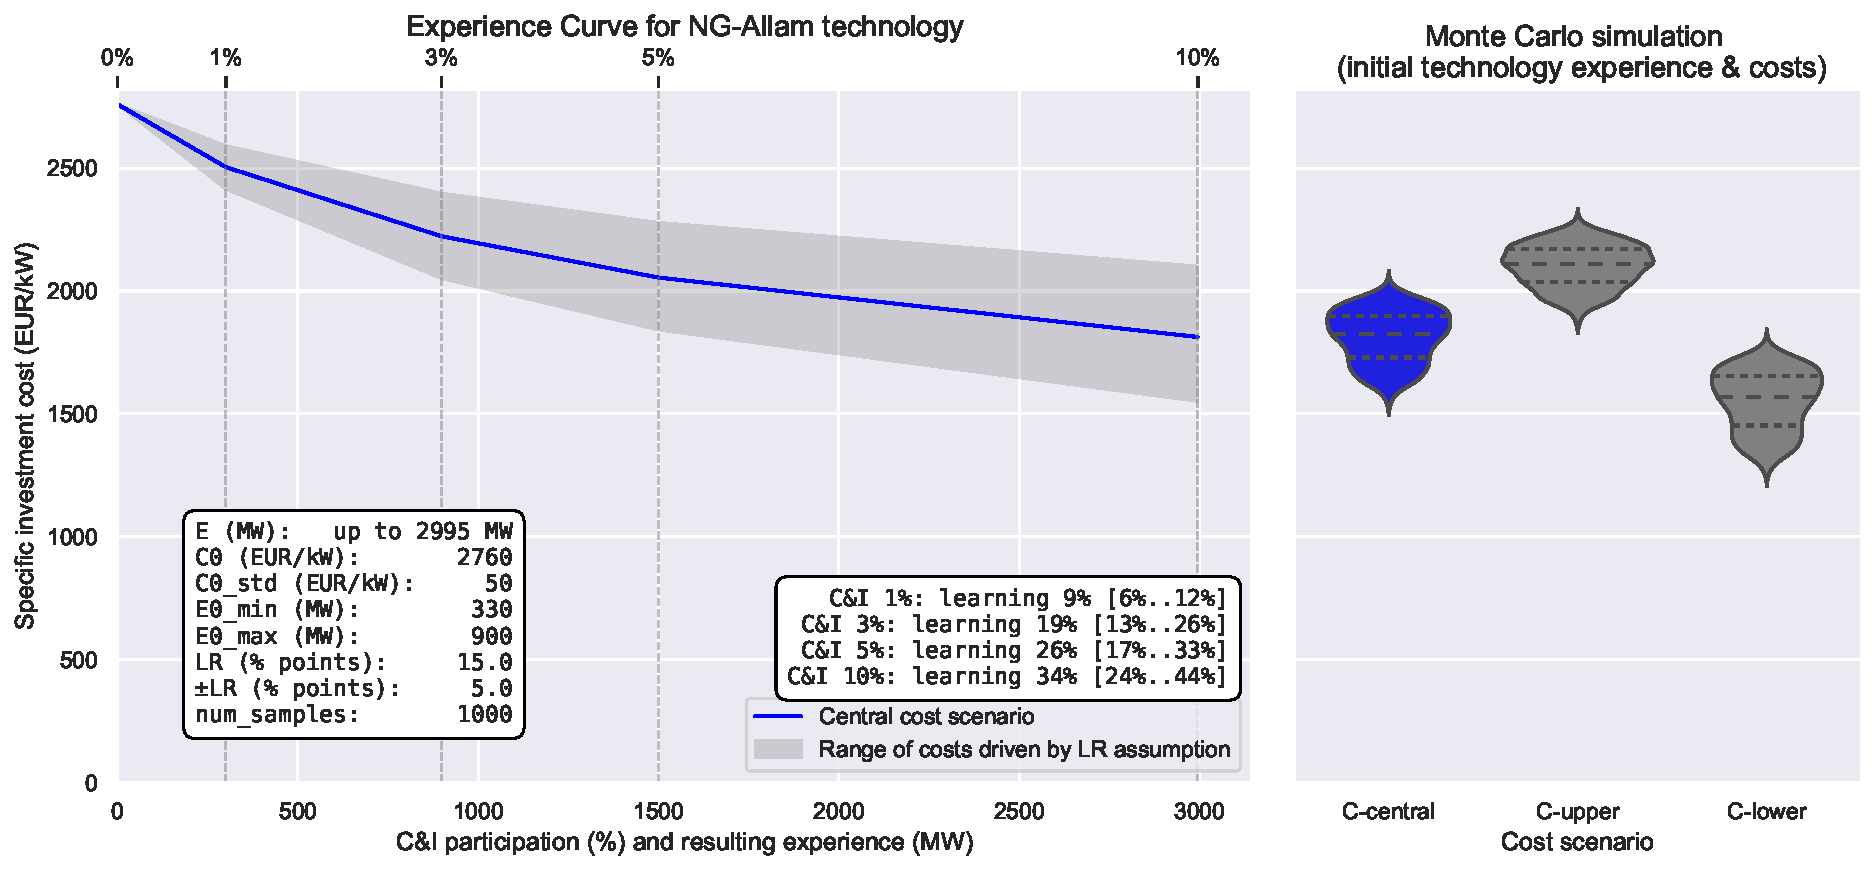
\includegraphics[width=\textwidth]{images/e_curve_NG-Allam.pdf}
    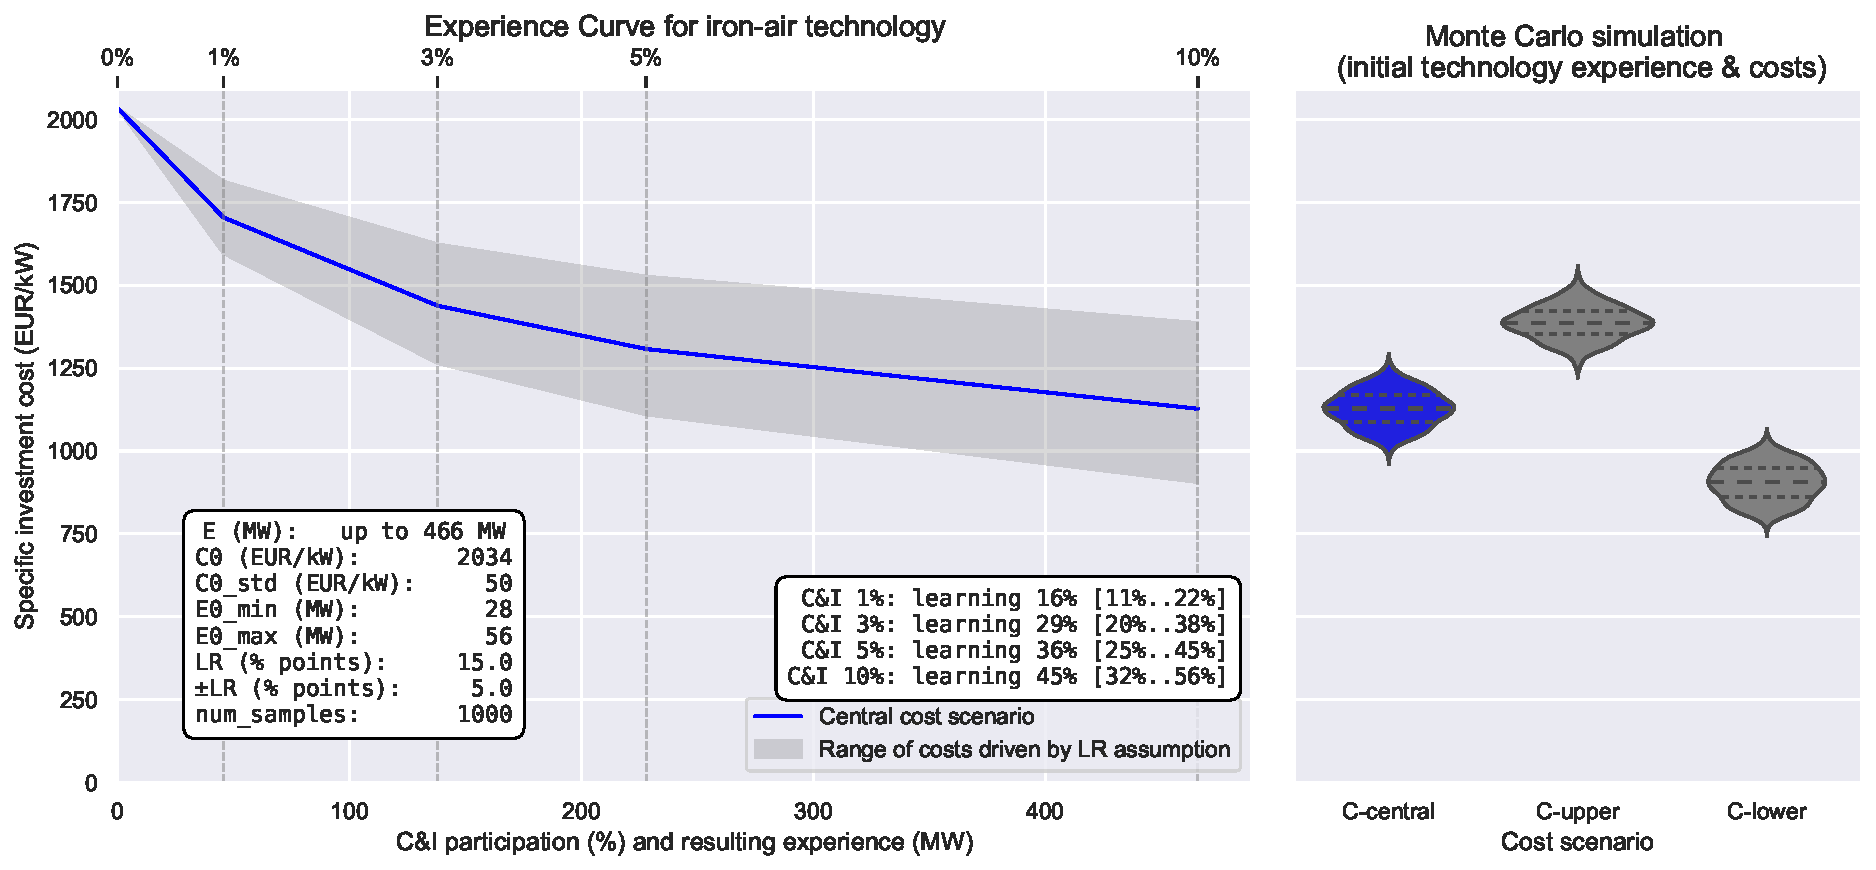
\includegraphics[width=\textwidth]{images/e_curve_iron-air.pdf}
    \caption{Technology learning curves for the NG-Allam cycle (\textbf{top panel}) and iron-air battery storage (\textbf{bottom panel}).
    The learning curves are based on the experience model with the technology investments based on 24/7 CFE model with varying C\&I participation level $[0\%..10\%]$ and learning rates of 15$\pm$5\% resembling a wide range of possible outcomes for modular energy technologies \cite{waySuppplementaryMaterialsEmpirically2022}. For the Monte Carlo analysis calibration, the initial costs (C0) are sampled from a normal distribution with a mean based on technology cost assumptions for 2025 and a standard deviation of 100~EUR/kW. Initial experience levels (E0) are sampled from a uniform distribution, with bounds derived from public information about planned projects. For the NG-Allam case, initial experience lies between cases when one of two projects planned by 2025 is completed, and when both projects are completed; for the iron-air case, the distribution bounds are formed by assuming that 50\% to 100\% of the projects announced to operate by 2025 are realized on time (more information about these projects is provided in Supplementary Information).
    }
    \label{fig:panels}
\end{figure}

\subsection*{Beyond directly reduced emissions}\label{sec4}

An illustration of the broader system impact is shown in Fig. \ref{fig:impact}, where we model the German electricity system in 2030 from a system planner's perspective. Here, we minimize the total system costs, including investment costs and operational costs of power generation and storage assets, while adhering to a set of operational constraints. For this case, we assume no voluntary commitments to CFE matching, meaning that power capacity investments are made solely on the basis of economic considerations. The four scenarios represent different levels of CAPEX for iron-air battery storage, starting from the baseline scenario with 2034 \officialeuro/kW, and reducing the cost by 25\% in each step. While we use a toy model representation of the German electricity system as an example, the system dynamics observed in simulations are generalizable to other markets and technologies. The same principles applied in multiple markets would indeed allow a wider palette of advanced technologies to be supported.

The results indicate that iron-air batteries need to cost around 1525 \officialeuro/kW to become economically competitive in the broader electricity system, which represents a 25\% reduction from the baseline. The learning model for iron-air storage shows that this level would require a quadrupling of iron-air capacity expected by 2025 (with a conservative assumption of LR$\sim$12\%, see Fig. \ref{fig:panels}). In other words, assuming that the first movers do not benefit from the learning effect, an investment of approx. \officialeuro340 million (168 [MW] $\cdot$ 2034 [\officialeuro/kW] $\cdot$ 1$^3$ [MW/kW]) can bring iron-air battery storage to the point of economic break-even by 2030, unlocking a wide range of societal benefits. To put this number in perspective, Germany paid approximately \officialeuro 1 billion for redispatch measures in 2023; the  costs of the Nord Stream 2 project is estimated at \officialeuro 9.5 billion. The unlocked benefits include reduced system emissions---as shown in Fig. \ref{fig:impact}, iron-air storage substitutes fossil peakers (gas open-cycle generators) reducing emissions in the electricity system by 3~MtCO$_2$ annually, already for a 25\% reduction in iron-air storage costs. There are other advantages of long-duration storage technology deployment beyond the focus of this analysis, such as reduced curtailment of wind and solar generation, reduced need for additional transmission infrastructure, and increased energy security.

Such learning effects can be achieved if a handful of companies and governments (an aggregate electricity demand of approx. 1200 MW---only 3\% of German C\&I electricity demand) target 24/7 CFE procurement and include advanced energy technologies in their portfolios (see Fig. \ref{fig:panels}). The required investment can be distributed among a wide range of actors since companies from various sectors and regions can join the movement and contribute to technology learning. Early adoption of advanced technologies will also lead to technology learning and cost reductions for other actors. It spins a \enquote{virtuous circle of innovation}, as we describe next.

\begin{figure}[htbp]
    \centering
    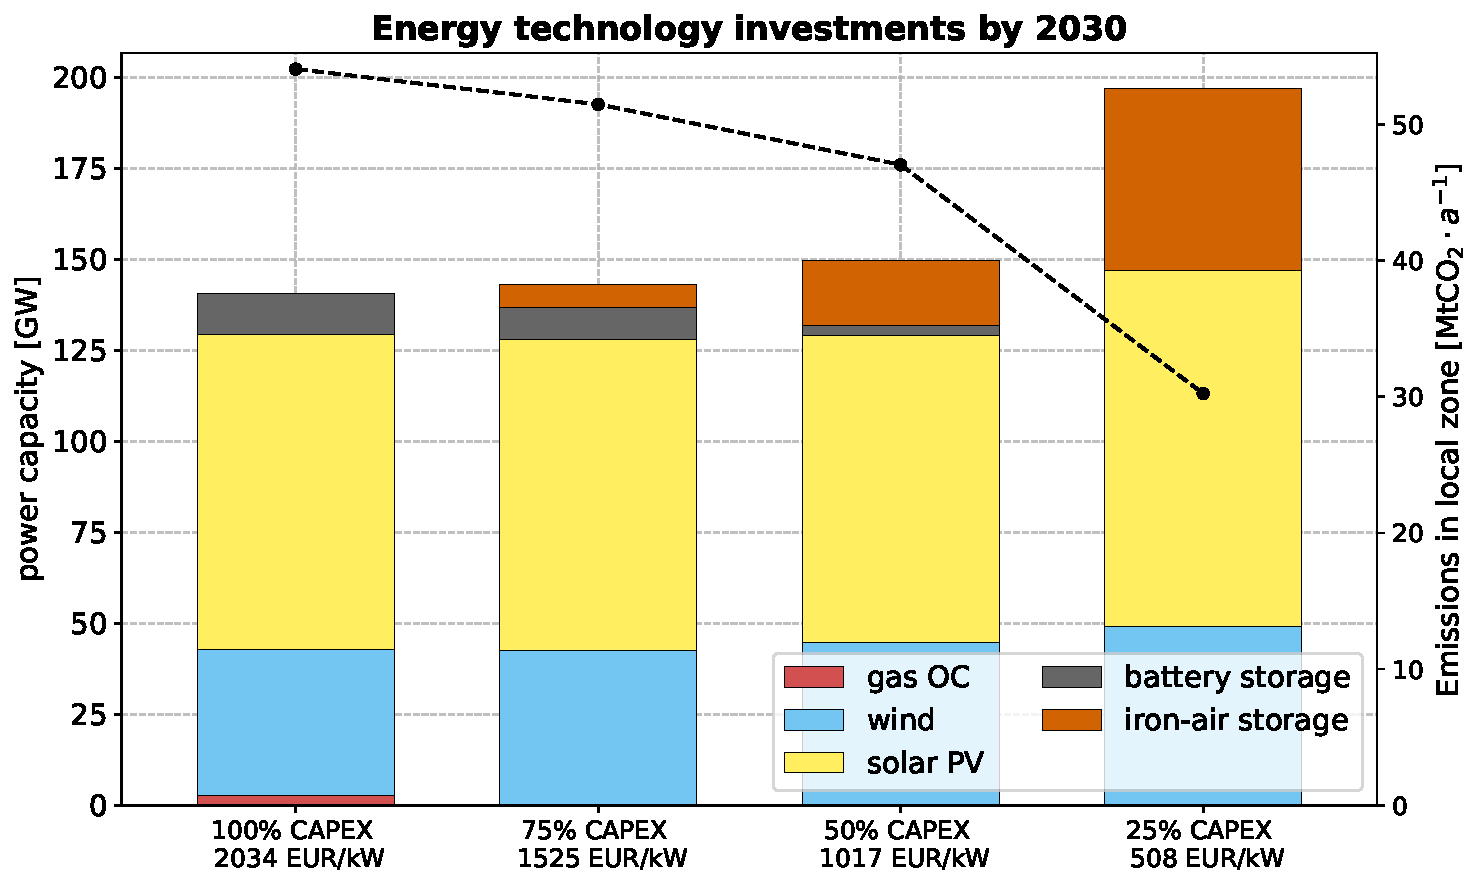
\includegraphics[width=0.8\textwidth]{images/dashboard_3.pdf}
    \caption{Power capacity investments and emissions in a toy model representation of German 2030 electricity system as a function of CAPEX for iron-air storage. Technology assumptions are provided in Supplementary Information. Price for EU ETS allowances is assumed to be 100 EUR/tCO$_2$. The configuration file in a public GitHub repository lists other background system assumptions \cite{code247CFE}.}\label{fig:impact}
\end{figure}

Note that this section presented a toy model exercise in the spirit of \enquote{modeling for insight} instead of \enquote{modeling for numbers} \cite{huntingtonModelingInsightsNot1982}. The back-of-the-envelope nature of this calculation does not aim at quantifying the learning effects of advanced energy technologies and their economical break-even points precisely.
It is rather a model experiment to illustrate that a relatively small number of electricity buyers who commit to 24/7 CFE can create a demand pull for advanced technologies, that is sufficient to kickstart learning effects and make new technologies more accessible and affordable for everyone.

\subsection*{A virtuous circle of innovation}\label{sec5}

24/7 CFE matching accelerates electricity system decarbonization through three channels: (1) directly reducing emissions during hours when procured CFE is matched with electricity consumption, (2) inducing learning effects that make 24/7 matching more attractive for other companies, and (3) enabling advanced energy technologies to become cost-competitive and widely adopted across the broader electricity system:

\begin{enumerate}
    \item The first channel comprises two mechanisms for directly reduced emissions. First, \enquote{profile} mechanism refers to participating buyers procuring CFE resources that match their demand patterns. When some consumers align their demand with CFE supply on an hourly basis, the rest of the electricity system requires less dispatchable generation to firm intermittent renewable supply. The utilisation of fossil-based generators, such as gas-fired power plants, is therefore reduced since participating consumers rely on procured CFE resources to cover their demand at all times. This reduces emissions associated with electricity consumption of participating buyers, as shown in Fig. \ref{fig:dashboard}.
    Second, a \enquote{volume} mechanism relates to the impact of excess CFE, i.e., clean electricity generated by 24/7 CFE portfolio that exceeds demand in a given hour can be sold to the grid to replace emitting grid generators. Both mechanisms are explained in detail by \citet{xu-247CFE-report} and \citet{riepinMeansCostsSystemlevel2024}.
    \item A second, indirect channel is the learning caused by early commitments to 24/7 CFE that facilitate innovation and create the early market for advanced technologies, as shown in Fig.~\ref{fig:panels}.
    This reduces the price premium for 24/7 CFE procurement goals, encouraging more companies to work towards them. This in turn further lowers system emissions via the two mechanisms in \#1.
    \item Finally, as advanced technologies are deployed repeatedly, they become economically competitive and are adopted more rapidly across the broader electricity system, thereby unlocking greenhouse gas savings beyond the directly reduced emissions associated the corporate portfolios in \#1 and \#2, as shown in Fig. \ref{fig:impact}. This channel is significant as the benefits extend beyond voluntary commitments to clean energy matching, affecting numerous actors in various regions and jurisdictions.
\end{enumerate}

% \begin{figure}[h]
%     \centering
%     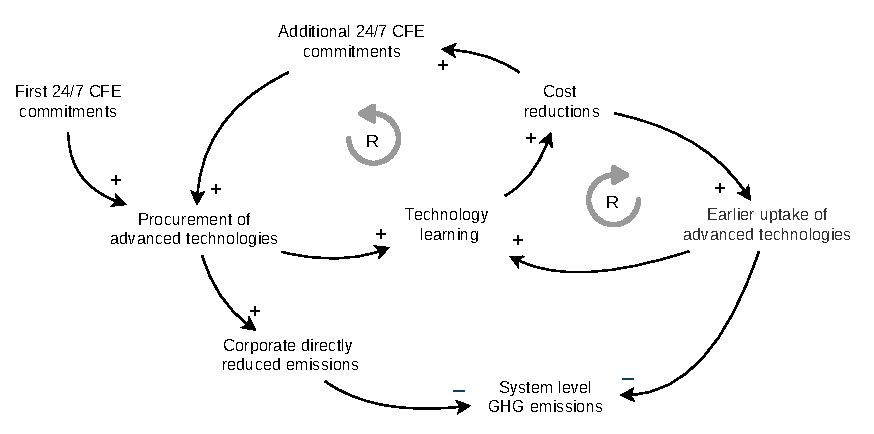
\includegraphics[width=0.9\textwidth]{images/virtuous_dynamics.pdf}
%     \caption{System dynamics of 24/7 CFE matching}\label{fig:dynamics}
% \end{figure}

A graphical abstract illustrates the nature of the system dynamics that result from initial commitments to 24/7 CFE. It is a self-reinforcing cycle where early commitments create a market for advanced clean energy technologies, thereby reducing the costs of hourly CFE matching and making it more attractive for other companies to join the movement. A second self-reinforcing cycle emerges when new technologies are adopted early in the electricity system, which further reduces system-level emissions and drives down costs for all actors in the system. The result is a \enquote{virtuous circle} that spurs innovation, financeability, and widespread availability of advanced energy technologies, thereby accelerating decarbonization of electricity systems.

This virtuous circle of innovation can be activated by a handful of companies and governments committed to timely action. The early-movers might be motivated to participate in 24/7 CFE through several incentives. First, corporate leadership campaigns can create strong incentives for action. Just as the RE100 campaign focused companies on 100\% annual matching and celebrated them for working towards it \cite{re100RE1002023Annual2024}, the 24/7 Carbon-free Coalition can increase commitments in the 24/7 CFE space. Additionally, companies may be motivated by the research-based evidence of the positive impacts of 24/7 CFE procurement on electricity decarbonization, including through spillover effects of advanced technology commercialization. Finally, increasing public and regulatory scrutiny on corporate sustainability claims and a trend toward greater accuracy in electricity carbon accounting---such as potential updates of the Greenhouse Gas Protocol Scope 2 Guidance to require more granular accounting---may encourage companies to move towards 24/7 CFE matching.

\subsection*{Takeaways}\label{sec6}

Early markets for advanced clean energy technologies can spur substantial technological learning, leading to cost reductions and unlocking greenhouse gas savings far beyond the reduction of emissions directly associated with initial investments.
Similarly to the feed-in tariffs and renewable portfolio standards that created a \enquote{demand pull} for wind and solar PV in the past, commitments to 24/7 CFE matching and other advance market commitments \cite{GoogleMicrosoftNucor} by private sector stakeholders can accelerate the development of first-of-a-kind and early commercial projects of innovative energy technologies.
A proactive private sector contribution can complement governmental support and reduce pressure on tight fiscal budgets.
The virtuous system dynamics we describe can be activated by a handful of companies and governments committed to timely action, thereby fostering rapid innovation and making climate solutions more accessible and affordable for everyone.

%%%%%%%%%%%%%%%%%%%%%%%%%%%%%%%%%%%%%%%%%%%%%%%%%%%%%%%%
\backmatter

\bmhead{Acknowledgements} We thank the following people for insights and fruitful discussions: Elisabeth Zeyen, Wilson Ricks, Adam Forni, Brian Denvir, Killian Daly, and the participants of the 24/7 CFE Hub Meeting in May 2024. IR and JJ acknowledge a research grant from Google LLC.

\bmhead{Author contributions}
\textbf{Iegor Riepin}: Conceptualization, Methodology, Formal analysis, Writing - Original Draft, Visualization
\textbf{Jesse D. Jenkins}: Conceptualization, Writing - Reviewing and Editing
\textbf{Devon Swezey}: Conceptualization, Writing - Reviewing and Editing
\textbf{Tom Brown}: Conceptualization, Validation, Supervision, Writing - Reviewing and Editing

\bmhead{Code availability} The code to reproduce the illustrative experiments is available at GitHub under open licenses \cite{code247CFE}.

\bmhead{Supplementary Information} Document S1. Table S1: Technology assumptions.Supplementary references.

\bibliography{sn-bibliography}% common bib file
%% if required, the content of .bbl file can be included here once bbl is generated
%%\input sn-article.bbl

\end{document}
